\documentclass{beamer}
\mode<presentation> {\usetheme{Madrid}}

\usepackage[utf8]{inputenc}
\usepackage{tikz}
\usepackage[export]{adjustbox}
\usepackage{amsmath}
\usepackage{appendixnumberbeamer}
\usepackage[absolute,overlay]{textpos}
\usepackage{subcaption}

\setbeamercolor{framesource}{fg=gray}
\setbeamerfont{framesource}{size=\tiny}
\setbeamertemplate{navigation symbols}{}
\setbeamercovered{transparent=00}
\setbeamerfont{footnote}{size=\tiny}

\newcommand{\todo}[1]{\textbf{\textcolor{red}{#1}}}
\newcommand{\td}[1]{\textcolor{gray}{#1}}
\newcommand{\bb}[1]{\textbf{#1}}
\newcommand{\me}[1]{\textcolor{gray}{#1}}
\newcommand{\source}[1]{\begin{textblock*}{4cm}(0.7cm,8.6cm)
	\begin{beamercolorbox}[ht=0.5cm,right]{framesource}
	\usebeamerfont{framesource}\usebeamercolor[fg]{framesource} Source: {#1}
	\end{beamercolorbox}
	\end{textblock*}
}

%%% TODO
% talk about why we use what chemical
% show recipe 2 zoomed in 
% thanks for your attention and open for questions and suggestions

\title[Insulating zirconia oxide layers on steel]{Status report: Insulating zirconia oxide layers on steel}
\author{Johann Dorn}
\begin{document}
%\date{\tomorrow}


%%%%% TITLEPAGE
\begin{frame}
 \titlepage
\end{frame}

\iffalse
\begin{frame}
 \frametitle{Overview \todo{just for me}}
	\begin{itemize}
		%\item chapter/todo
		\item what is the goal? which project?
		\item goal: make continuous insulation layer from non-toxic materials which is scalable
		\item this should be a layer between an steel foil and a silicon layer
		\item starting solution was slightly optimized from M A Anwar et al 2017 [1]
		\item what did we vary
		\item what were the outcomes (SEM) -> bad bcs of cracks
		\item looks like in paper, not bcs of lack of control \& consistency but bcs of recipe
		\item other literature as starting point (Hu et al. 2016) [2]
		\item spin coating and Al2O3: adapt
		\item result of new recipe (SEM)
		\item outlook:
		\item make layer thicker, 
		\item minimize production time
		\item adapt to make scaleable
		%%%%%% new
		\item talk about project: objective/ application
		\item what kind of insulating coatings
		\item how do we make the coatings
		\item oulook: \~100nm layer, dielectric properties I-V, C-V, printing contacts
		\item XRD
		\item optical spectrometry
	\end{itemize}
\end{frame}
\fi

\begin{frame}
	\frametitle{Introduction}
	\begin{itemize}
		\item Project: \textbf{InnovaSteel4CIGS} (AIT - Sunplugged)
		\item \bb{C}opper\bb{I}ndium\bb{G}allium\bb{S}elenide
		\item Objective: 
			\begin{itemize}
				\item Insulating coating for stainless steel
				\item ZrO$_2$ and/or Al$_2$O$_3$
				\item Scalability for industry
			\end{itemize}
		\item application: insulation between CIGS cell and steel foil

%		\item \bb{C}opper\bb{I}ndium\bb{G}allium\bb{S}elenide
%		\item \me{pic of CIGS cell }
	\end{itemize}
	%\pause
	\begin{figure}
		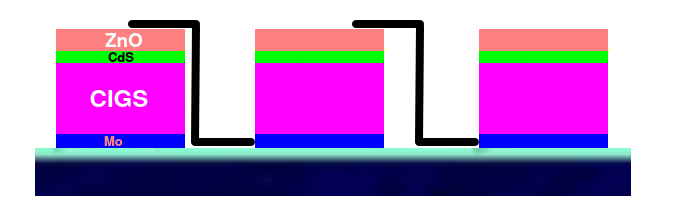
\includegraphics[width=\textwidth]{Images/cigs_mod.png}
	\end{figure}
\end{frame}

\begin{frame}
	\frametitle{Starting point}
	\centering{
	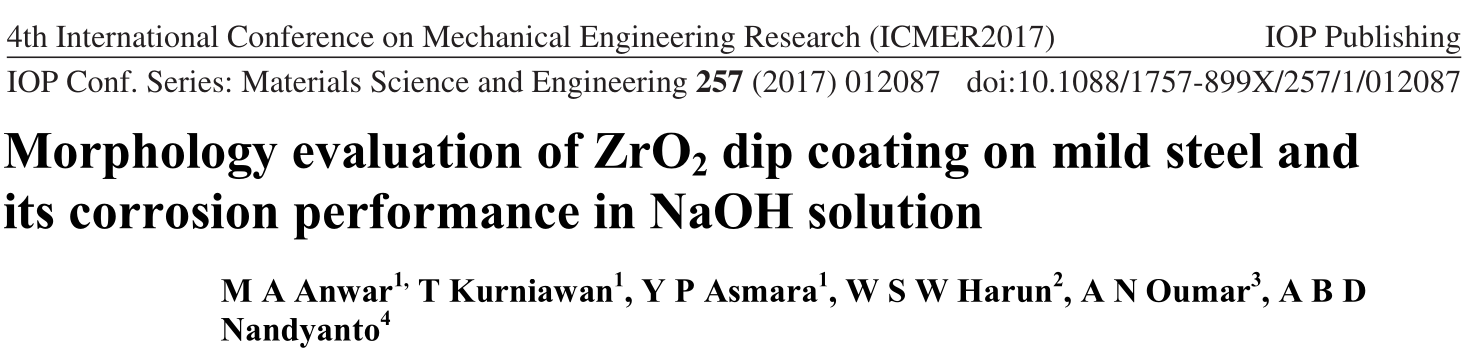
\includegraphics[width=\textwidth]{Images/zro2.png}
	\includegraphics<1>[width=.9\textwidth]{Images/cracks50.png}
%	\includegraphics<2->[width=.9\textwidth]{Images/cracks20.png}
}
\end{frame}

\begin{frame}
	\frametitle{Recipe and Parameters}
	\begin{columns}[t]
		\column{0.39\textwidth}
			\textbf{Recipe 1:}
			\begin{itemize}
				\item 8ml Zr(OPr)$_4$
				\item 8ml AcAc 
				\item 2ml i-PrOH
				\item 2.6ml H2O
			\end{itemize}
			\visible<2->{\textbf{Parameters:}}
			\begin{itemize}
				\item<2-> Heating rate 
				\item<2-> calcination temperature
				\item<2-> Mixing time
				\item<2-> pH regulator
				\item<2-> Surfactant
				\item<2-> High molecular polymer
			\end{itemize}
		\column{0.59\textwidth}
			\begin{figure}
				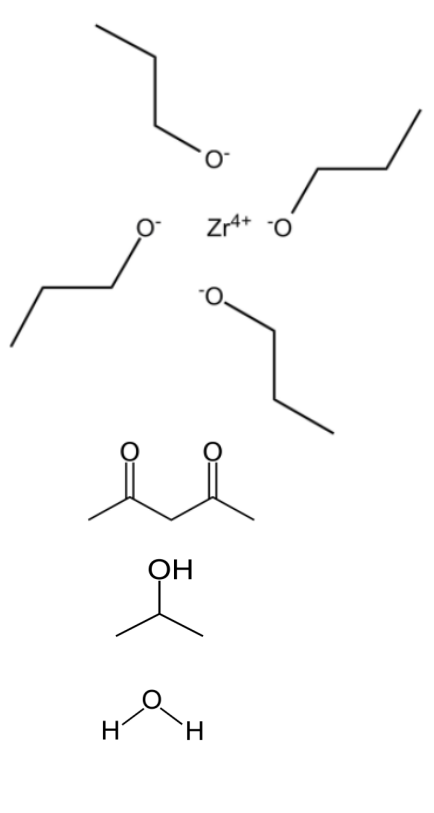
\includegraphics[height=0.8\textheight]{Images/recipe1.png}
			\end{figure}
	\end{columns}
\end{frame}

\begin{frame}
	\frametitle[center]{SEM results}
	\begin{figure}
		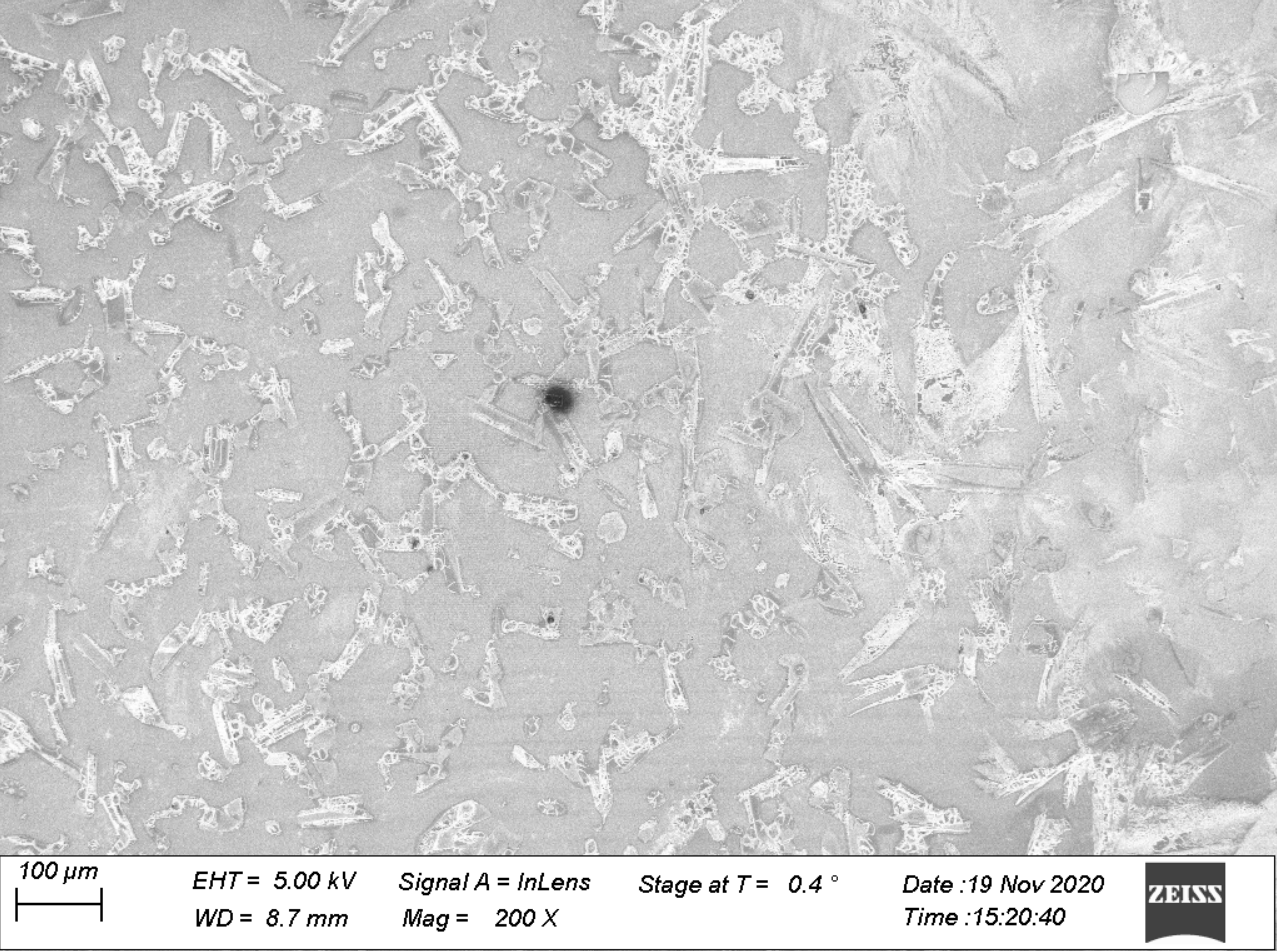
\includegraphics[width=0.4\textwidth]{Images/r1_sem_200.png}
		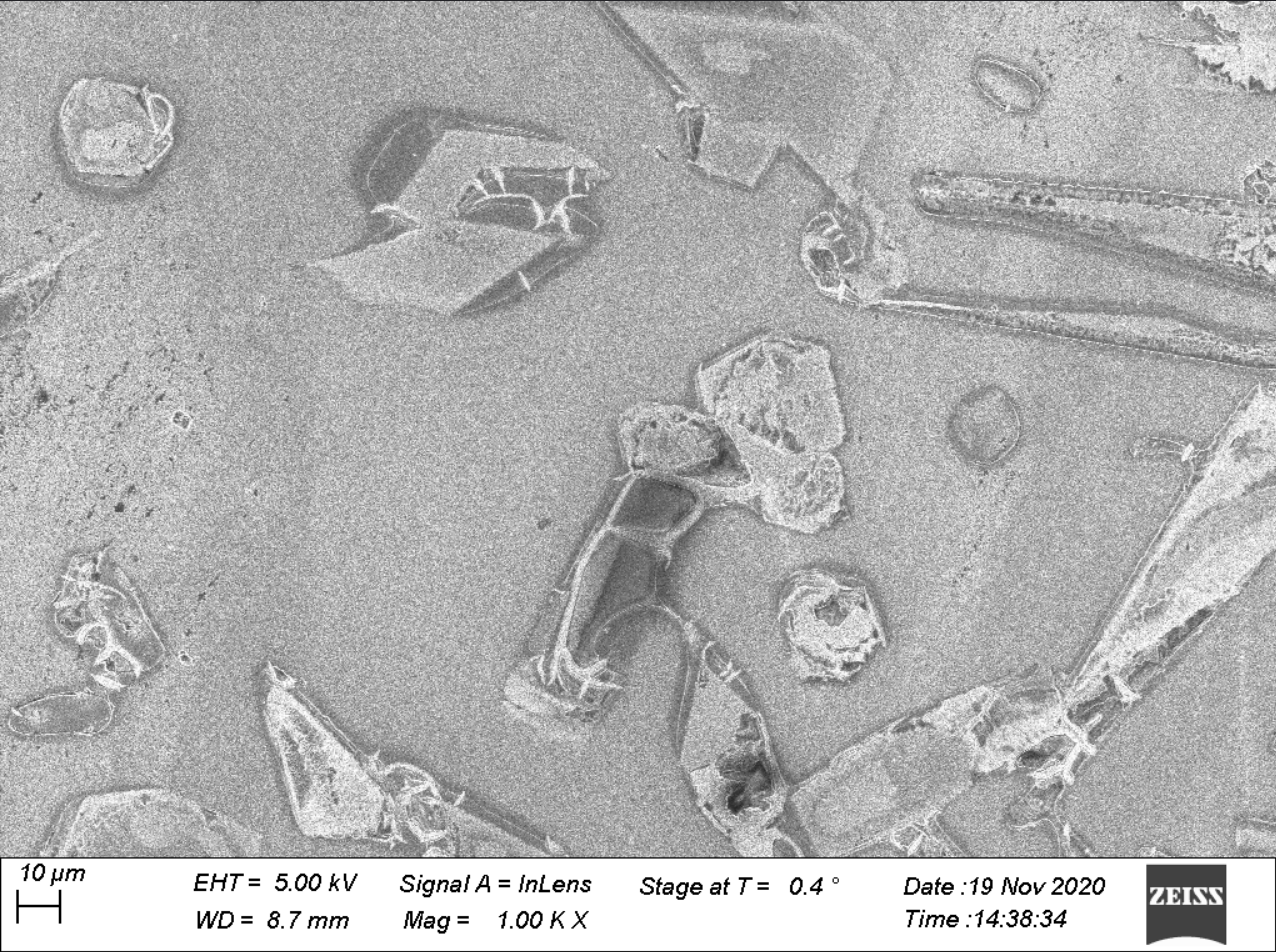
\includegraphics[width=0.4\textwidth]{Images/r1_sem_1k.png}
%		\pause
		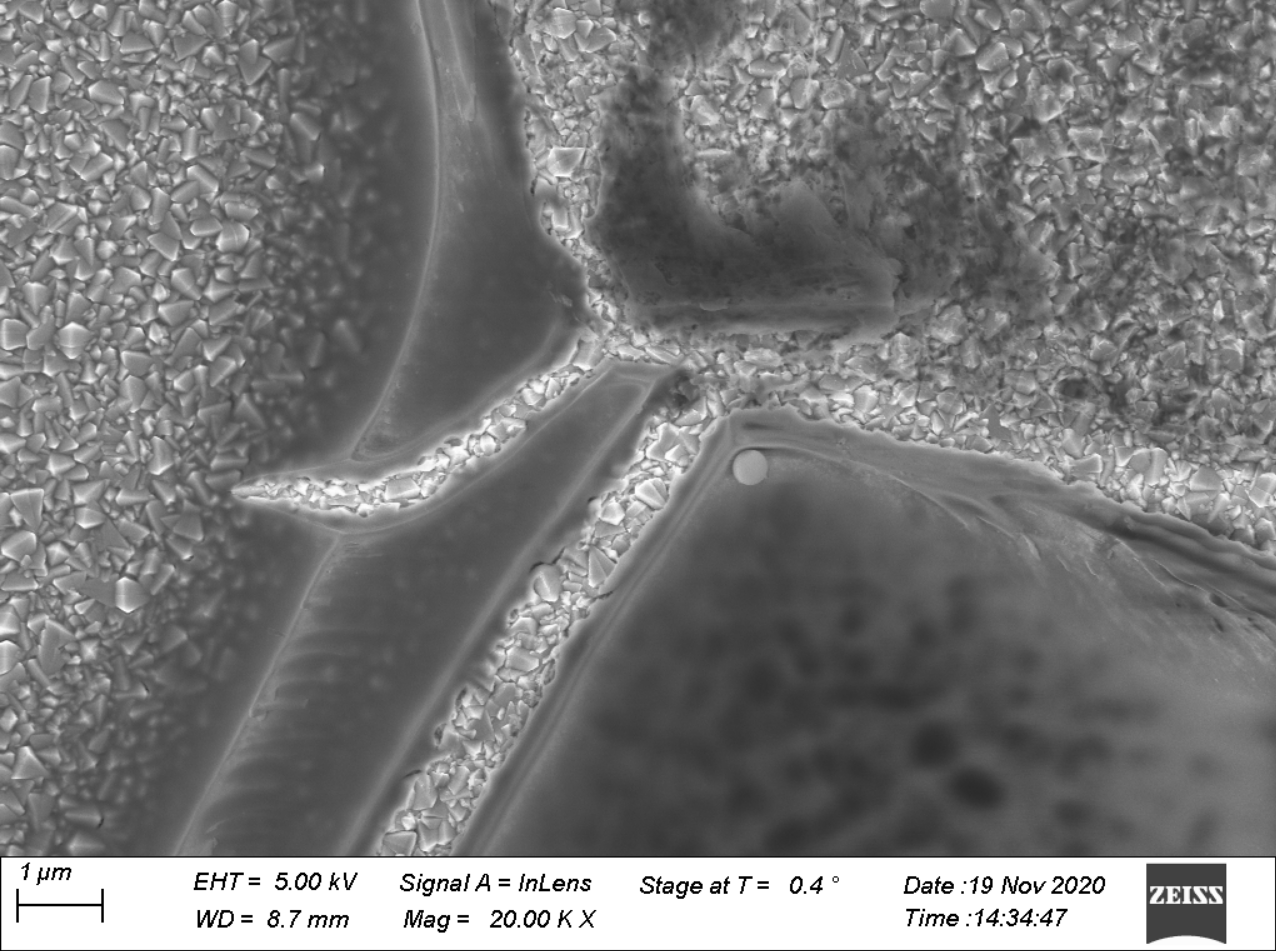
\includegraphics[width=0.4\textwidth]{Images/r1_sem_20k.png}
		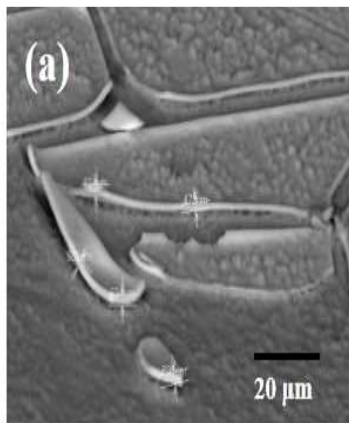
\includegraphics[width=0.25\textwidth]{Images/cracks20_single.png}
	\end{figure}
\end{frame}

\begin{frame}[t]
	\frametitle{Adapted recipe 2}
	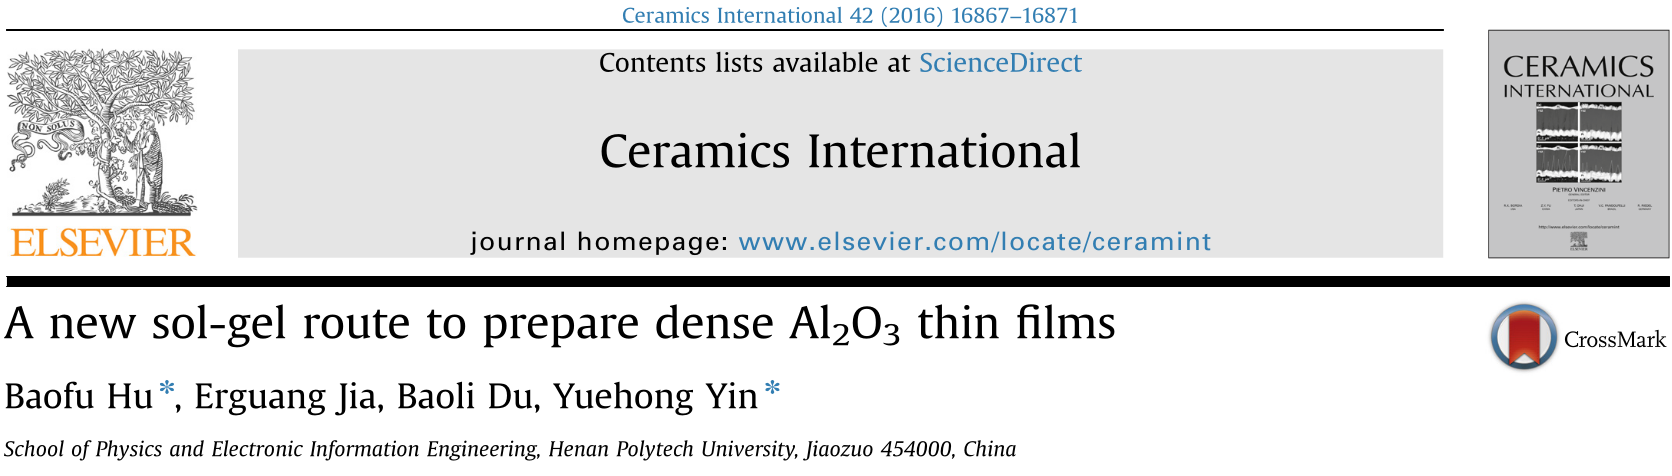
\includegraphics[width=0.99\textwidth]{Images/a2o3.png}
	\begin{columns}[t]
		\column{0.29\textwidth}
			\textbf{Recipe 2:}
			\begin{itemize}
				\item 9.9ml 1-BuOH
				\item 0.1ml Zr(OPr)$_4$
				\item 0.025 AcAc
				\item 2ml AcOH
			\end{itemize}
		\column{0.69\textwidth}
			\begin{figure}
				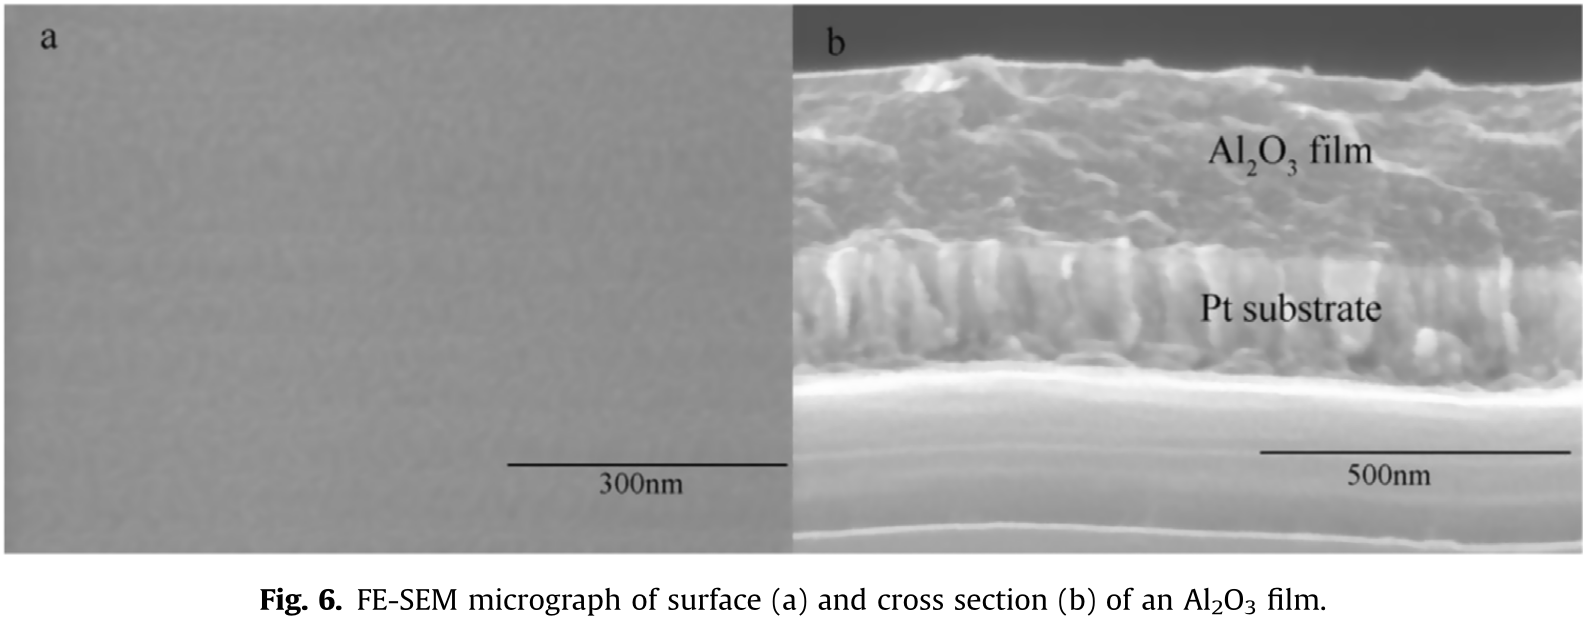
\includegraphics[width=\textwidth]{Images/nocracks.png}
			\end{figure}
			\vfill

	\end{columns}
\end{frame}

\begin{frame}
	\frametitle{SEM results }
	\begin{figure}
		\begin{subfigure}{.49\textwidth}
		\centering
			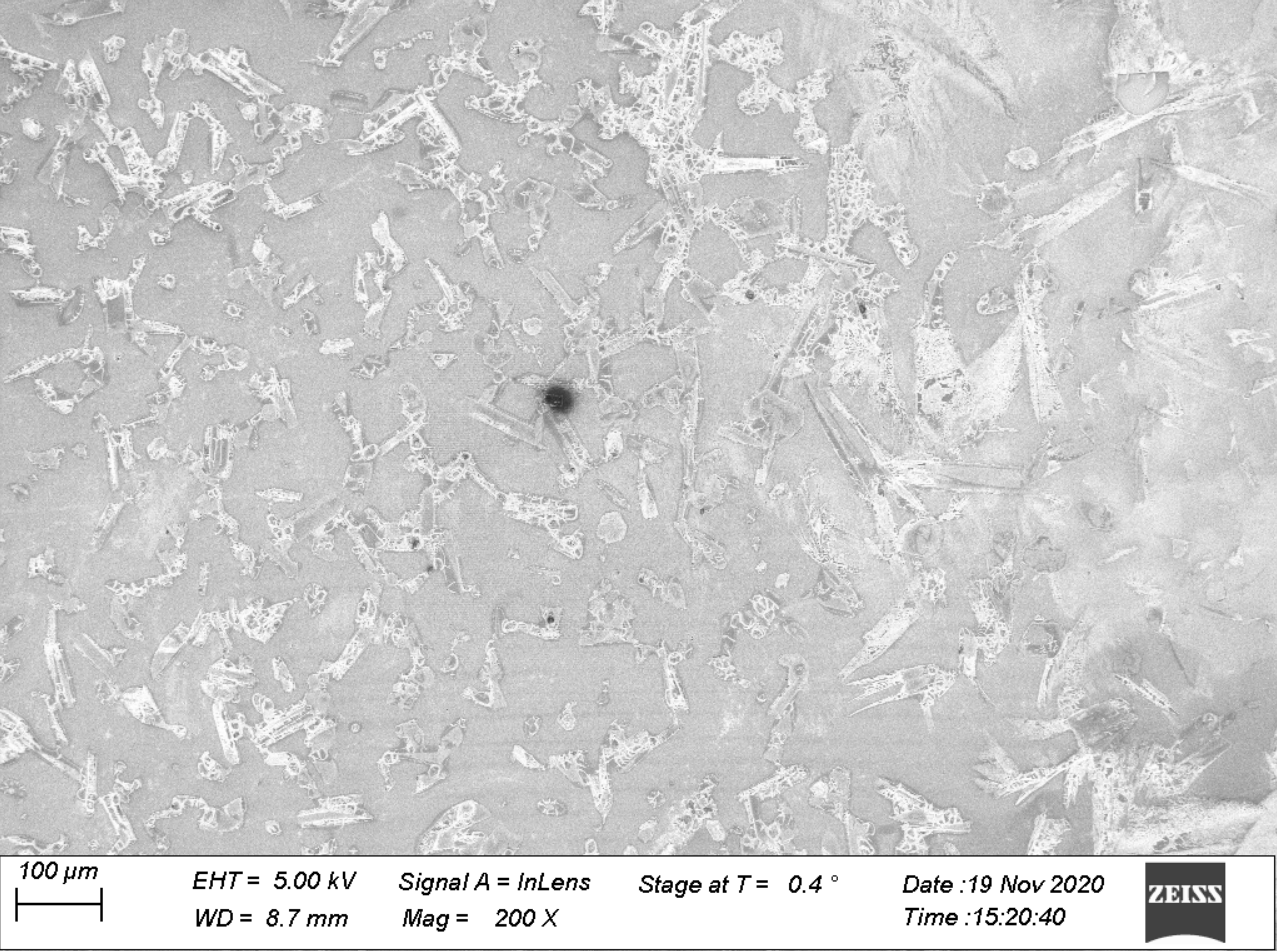
\includegraphics[width=0.9\textwidth]{Images/r1_sem_200.png}
			\caption{Recipe 1}
		\end{subfigure}
		\begin{subfigure}{.49\textwidth}
		\centering
			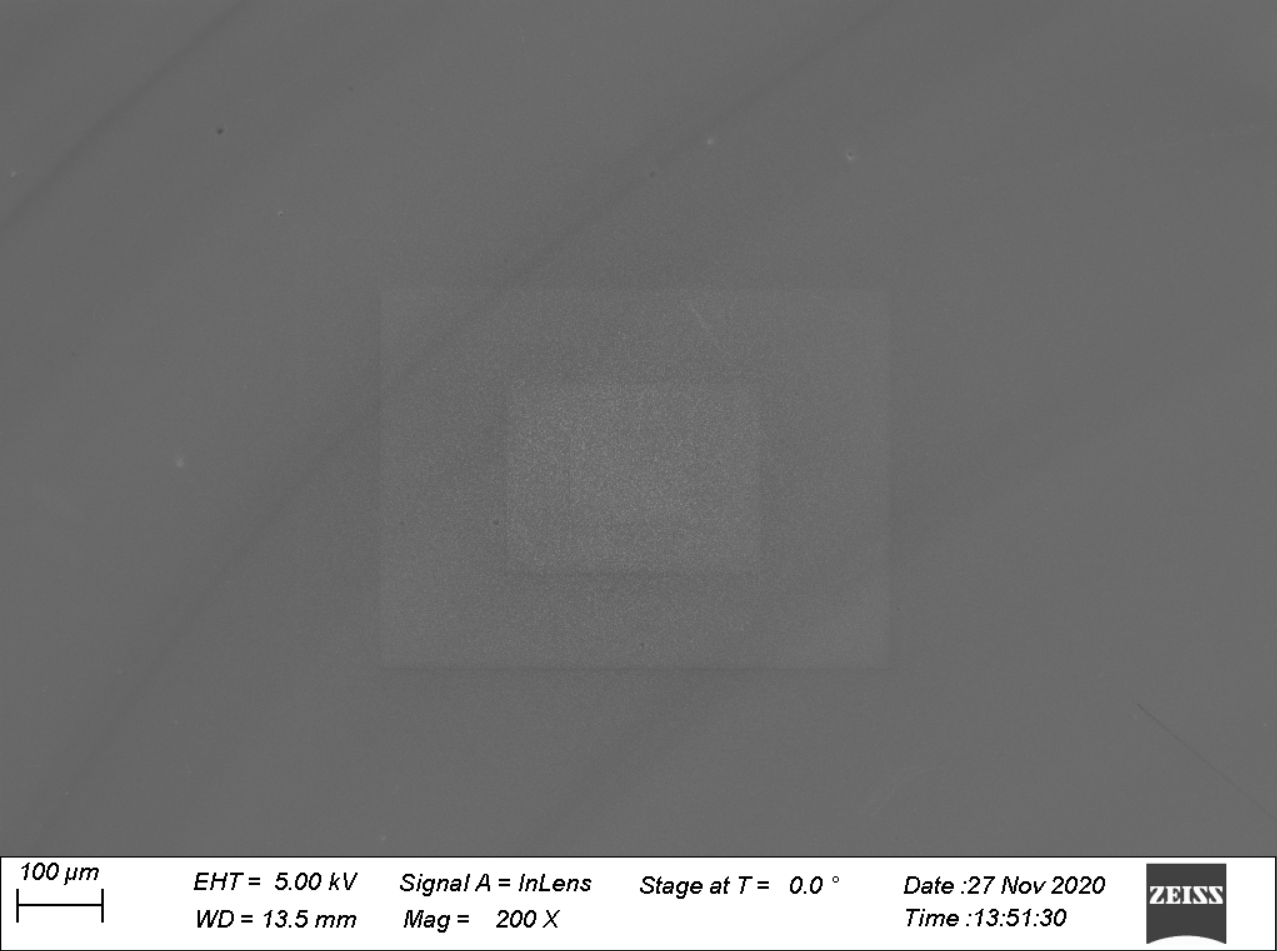
\includegraphics[width=0.9\textwidth]{Images/r2_sem_200.png}
			\caption{Recipe 2}
		\end{subfigure}
	\end{figure}

\end{frame}

\begin{frame}
	\frametitle{SEM cross section }
	\begin{figure}
		\centering
		%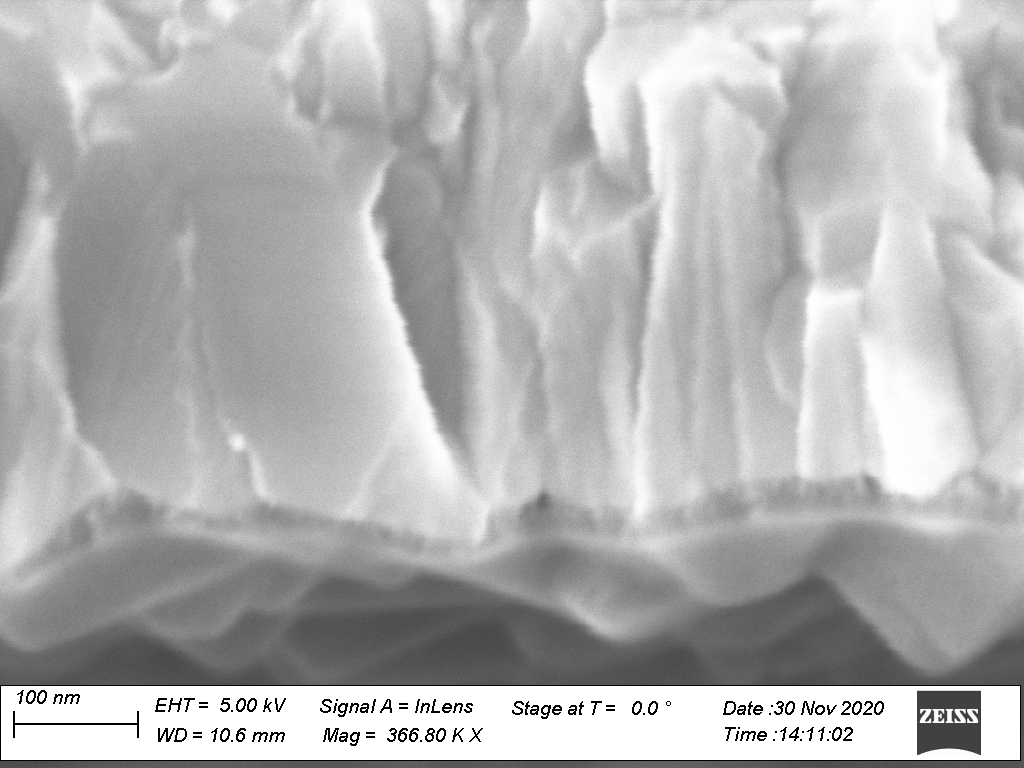
\includegraphics[width=.95\textwidth]{Images/buac_cs.png}
		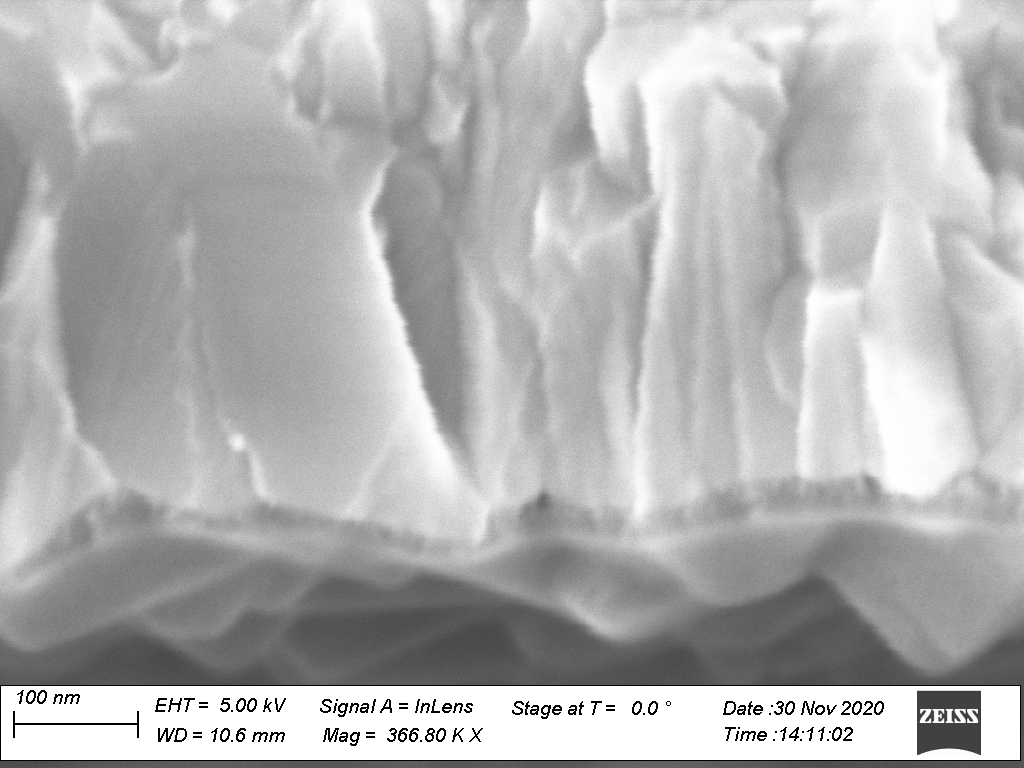
\includegraphics[height=.85\textheight]{Images/buac_cs.png}
		\caption{Recipe 2}
	\end{figure}
\end{frame}

\begin{frame}
	\frametitle{Summary and Outlook}
		\begin{itemize}
			\item 100nm layer
%			\item minimize production time 
%			\item adapt to make scalable
%			\item confirm that it is insulating
			\item dielectric properties: I-V, C-V
			\item optical spectrometry
			\item XRD
			\item Machine Learning
		\end{itemize}
\end{frame}
\iffalse 
\begin{frame}
	\frametitle{Summary and Outlook}
	\begin{columns}[t]
		\column{0.49\textwidth}
			\begin{itemize}
				\item second approach produces continuous layer
			\end{itemize}
		\column{0.49\textwidth}
			\begin{itemize}
				\item make layer thicker 
				\item minimize production time 
				\item adapt to make scalable
				\item confirm that it is insulating

			\end{itemize}
	\end{columns}
\end{frame}
\fi


%%%%%%%%%%%%%%%%%%%%%%%%%%%%%%%%%%%%%%%%%%%%%%%%%%%%%%%%%%60
\iffalse
\appendix
\begin{frame}
	\frametitle{Frequency Dependence of Permitivity}
	\begin{block}{Blocktitle}
	\end{block}
	\begin{enumerate}
		\item void
	\end{enumerate}
	\begin{columns}[t]
		\column{0.49\textwidth}
		\begin{itemize}
			\item some thing
		\end{itemize}

		\column{0.49\textwidth}
		\begin{figure}
			\includegraphics[width=.5\textwidth]{example-image}
			\source{ACS Nano 2019, 13, 1177-1182}
		\end{figure}
	\end{columns}
\end{frame}

\begin{frame}
	\frametitle[center]{Single Walled Carbon Nano Tubes (SWCNT)}
	\begin{columns}[t]
		\column{0.49\textwidth}
		\begin{figure}
			\includegraphics<1>[width=.9\textwidth]{example-image-a}
			\includegraphics<2->[width=.9\textwidth]{example-image-b}
			\source{source}
		\end{figure}
	\column{0.49\textwidth}
		\begin{figure}
			\includegraphics<3->[width=.9\textwidth, right]{example-image-c}
		\end{figure}
		\pause
		\visible<4>{(3,1) SWCNT}
	\end{columns}
\end{frame}
\fi

\end{document}
